\clearpage
\section{Theoretical motivation\label{sec:theory}}

\subsection{The Standard Model\label{sec:SM}}

Particle physics concerns itself with the study of particles and the 
forces between them. Our current knowledge of their characteristics and 
interactions is formalized in the quantum field theory called the Standard Model 
(SM)~\cite{bettini2014introduction,griffiths2008introduction}.
It describes ``matter'' particles of spin-1/2 known as 
fermions. Six fermions of relatively small mass (leptons, $l$) are described:
the electrically charged electron ($e$), muon ($\mu$), and tau ($\tau$) 
leptons, and the electrically neutral and massless neutrinos 
$\nu_{e}$, $\nu_{\mu}$, $\nu_{\tau}$.  
Six other electrically charged 
fermions, named quarks, are in the Standard Model: up ($u$), down ($d$), 
charm ($c$), strange ($s$), top ($t$), and bottom ($b$). The quarks also carry
a charge analogous to the electric charge called color charge. Quarks in a 
free state have not been observed; they combine to make composite
particles called hadrons (e.g. protons, neutrons, pions). The masses of the 
fermions range from very small masses for neutrinos up to the heaviest 
particle described in the SM, the top quark, with a mass near 170 GeV. \\
\indent The interaction between these particles are mediated by spin-1 bosons: 
the massless and neutral photon $\gamma$ which mediates the electromagnetic force, 
the massive $W^\pm$ and $Z^0$ that mediate the weak force, and the eight color 
charged, electrically neutral massless gluons which mediate the strong force.

\begin{figure}[h!t]
  \begin{center}
       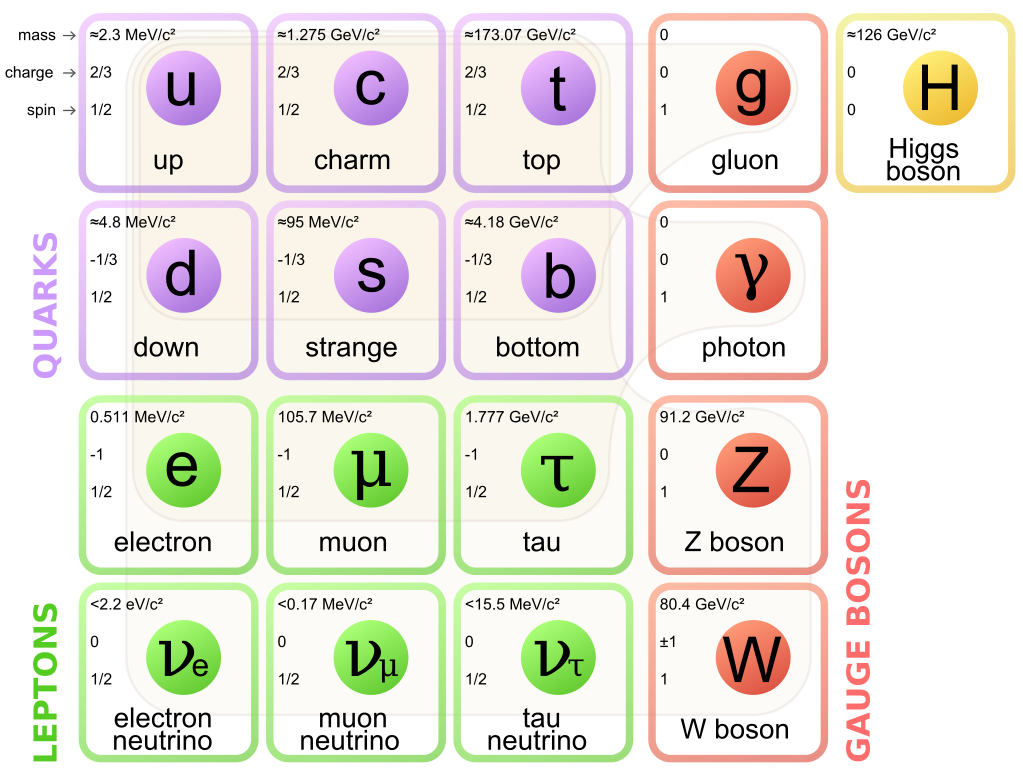
\includegraphics[width=0.85\textwidth,]{figures/Standard_Model_of_Elementary_Particles.png}
       \caption{The particles of the Standard Model.}
    \label{fig:SM-particles}
  \end{center}
\end{figure}

The interactions are governed by three symmetries of the SM: the color charge 
symmetry of Quantum Chromo Dynamics (QCD) represented in SU(3), the flavor 
symmetry of Quantum Flavor Dynamics (QFD) represented in SU(2) and the electric 
charge symmetry of Quantum Electro Dynamics represented in U(1). Together, SU(3) 
$\times$  SU(2) $\times$ U(1) requires the SM Lagrangian be invariant under 
local gauge transformations~\cite{perkins2000introduction}. The SU(2) $\times$ U(1) represent the electroweak interaction, 
which give rise to the photon, and the three weak gauge bosons: $W^{+}$, $W^{-}$ and $Z^0$.
%In the initial electroweak theory four massless bosons were introduced: $W^\pm$, $W^{0}$, $B^{0}$.
%Through the quantum numbers weak isospin $T$ and hypercharge $Y$, these bosons interact with all fermions.
The strength of the coupling between a boson and a fermion is determined by the 
charge belonging to the interaction. The quantum number weak isospin ($T$) is the charge 
of the weak interaction, and all interactions conserve the third component of weak isospin ($T_{3}$).
The electric charge ($Q$) can be represented by $T_{3}$ and the weak hypercharge ($Y$) 
corresponding to the U(1) symmetry:

\begin{equation}
\label{eq:Q-charge}
Q = T_{3} + \frac{Y}{2}
\end{equation}

Given the electroweak interaction is of the group SU(2) x U(1), there are four fields associated 
with it: $W_{1}$, $W_{2}$, $W_{3}$ of the SU(2) group where each index
corresponds to a component of the weak isospin space, and the isosinglet $B$ corresponding
to the weak hypercharge of the SU(1) group. These four objects, being vectors, require an index but it 
is dropped here for simplicity. The vectors $W_{1}$ and $W_{2}$ which result from the 
gauge invariance of the SU(2) group, mix to give rise to the $W^{\pm}$:

\begin{equation}
\label{eq:vector-boson}
W^{\left(\pm\right)}= \frac{1}{\sqrt{2}}\left(W_{1} \pm iW_{2}\right).
\end{equation}

The mixing of $W_{3}$ and $B$ give rise to the photon and $Z$ boson: 
$\gamma = B \cos \theta_W + W_{3} \sin \theta_W$  and $Z = W_{3}\cos \theta_W - B \sin \theta_W$ ,
where $\theta_W$ is the weak mixing angle. An exact symmetry does not allow mass 
terms in the Lagrangian because they are not invariant under a gauge transformation.
Since the gauge bosons of the weak interaction are not massless the symmetry must be broken.
This symmetry breaking also gives mass to the fermions of the SM. To parametrize the symmetry 
breaking a doublet of scalar complex fields is introduced, the so-called
Higgs field:
\begin{equation}
\label{eq:higgs-field}
\phi = \binom{\phi^{+}}{\phi^{0}}
\end{equation}

the potential is:
\begin{equation}
\label{eq:higgs-potential}
V(\phi) = \mu^2|\phi|^2 + \lambda|\phi|^2
\end{equation}

If $\mu^2 < 0$ and $\lambda > 0$ this leads to a non zero vacuum expectation value. 
As the field is described by a complex doublet it possesses four degrees of freedom. 
Three yield the mass of the weak gauge bosons. Since the fourth degree of freedom is 
not absorbed by the massless photon it results in a neutral spin-0 boson whose couplings 
to the fermions are proportional to their masses. This boson is named the Higgs boson and
its existence was recently confirmed by the CMS and ATLAS experiments at CERN.
Figure~\ref{fig:SM-particles} show the particles described in the SM along with their properties.

\subsection{Shortcomings of the SM}
The agreement between experimental measurements and SM predictions make
the theory incredibly successful. For example, the prediction of the anomalous magnetic dipole 
moment of the electron agrees to the \textit{billionth} decimal place with experimental 
measurement. Additionally, the SM prediction of the existence of the W, Z and Higgs boson
years (even decades) before their detection highlights its predictive power. Yet, the SM is not 
a complete theory. The observation of neutrino oscillation in the late 90's forced the first 
``Beyond the Standard Model'' (BSM) extension of the theory in order to give neutrinos 
mass~\cite{zuber2003neutrino}. Furthermore, gravitational interactions are not incorporated in the theory,
and therefore, at the scale which gravitational forces become non-negligible 
($\approx 10^{19}~\GeV$) the SM fails to make any predictions. Additionally, a theoretical 
framework explaining the dark matter in the universe is absent in the Standard Model.
But perhaps most importantly, within the SM, the Higgs mass ($m_{H}$) is corrected by fermionic
loop interactions which depend quadratically on the momentum cut-off scale, i.e. the scale 
which new physics may enter to alter the high-energy behavior of the theory~\cite{Martin:1997ns}.
A few problems arise. First, some of the parameters in the SM are suspiciously large, rather one 
would expect the parameters be close to 1 in natural units. Second, the parameters
need to be incredibly fine-tuned for the SM to properly predict experimental measurements of the
Higgs mass. Small deviations from these parameters results in very large fluctuations of the mass. 
Third, there is no clear formulation why the Higgs mass should be near the weak scale ($\sim\!250\gev$) 
and not closer to the Planck scale ($10^{19}\gev$). While not everyone will agree on the 
severity of these problems, it is generally agreed that any proposed addition to the SM 
(e.g. supersymmetry) should at least provide a mechanism to remove the quadratic divergence from the corrections of 
the Higgs mass.
%Any Such a quadratic dependence on the cut off is ivergence
%This huge ($\mathcal{O}$(1~TeV), quardatic divergence is 
%This divergence $\mathcal{O}$(1~TeV), 
%The SM has no mechanism to remove this quadratic divergence, yet the mass of th Higgs has been
%measured, therfore, and fine-tuned to it seems that nature  
%The fact that this correction is quardatic in nature, and not logarithmic like for 
%other particles, implies that for the newly measured Higgs mass of $\sim\!125~\gev$
%either new physics enters at the scale of $\mathcal{O}$(1 TeV), or some new
%mechanism is required to remove this quadratic divergence, $e.g.$ supersymmetry~\cite{Martin:1997ns}.

\subsection{Supersymmetry\label{sec:SUSY}}

\begin{figure}[h!t]
  \begin{center}
       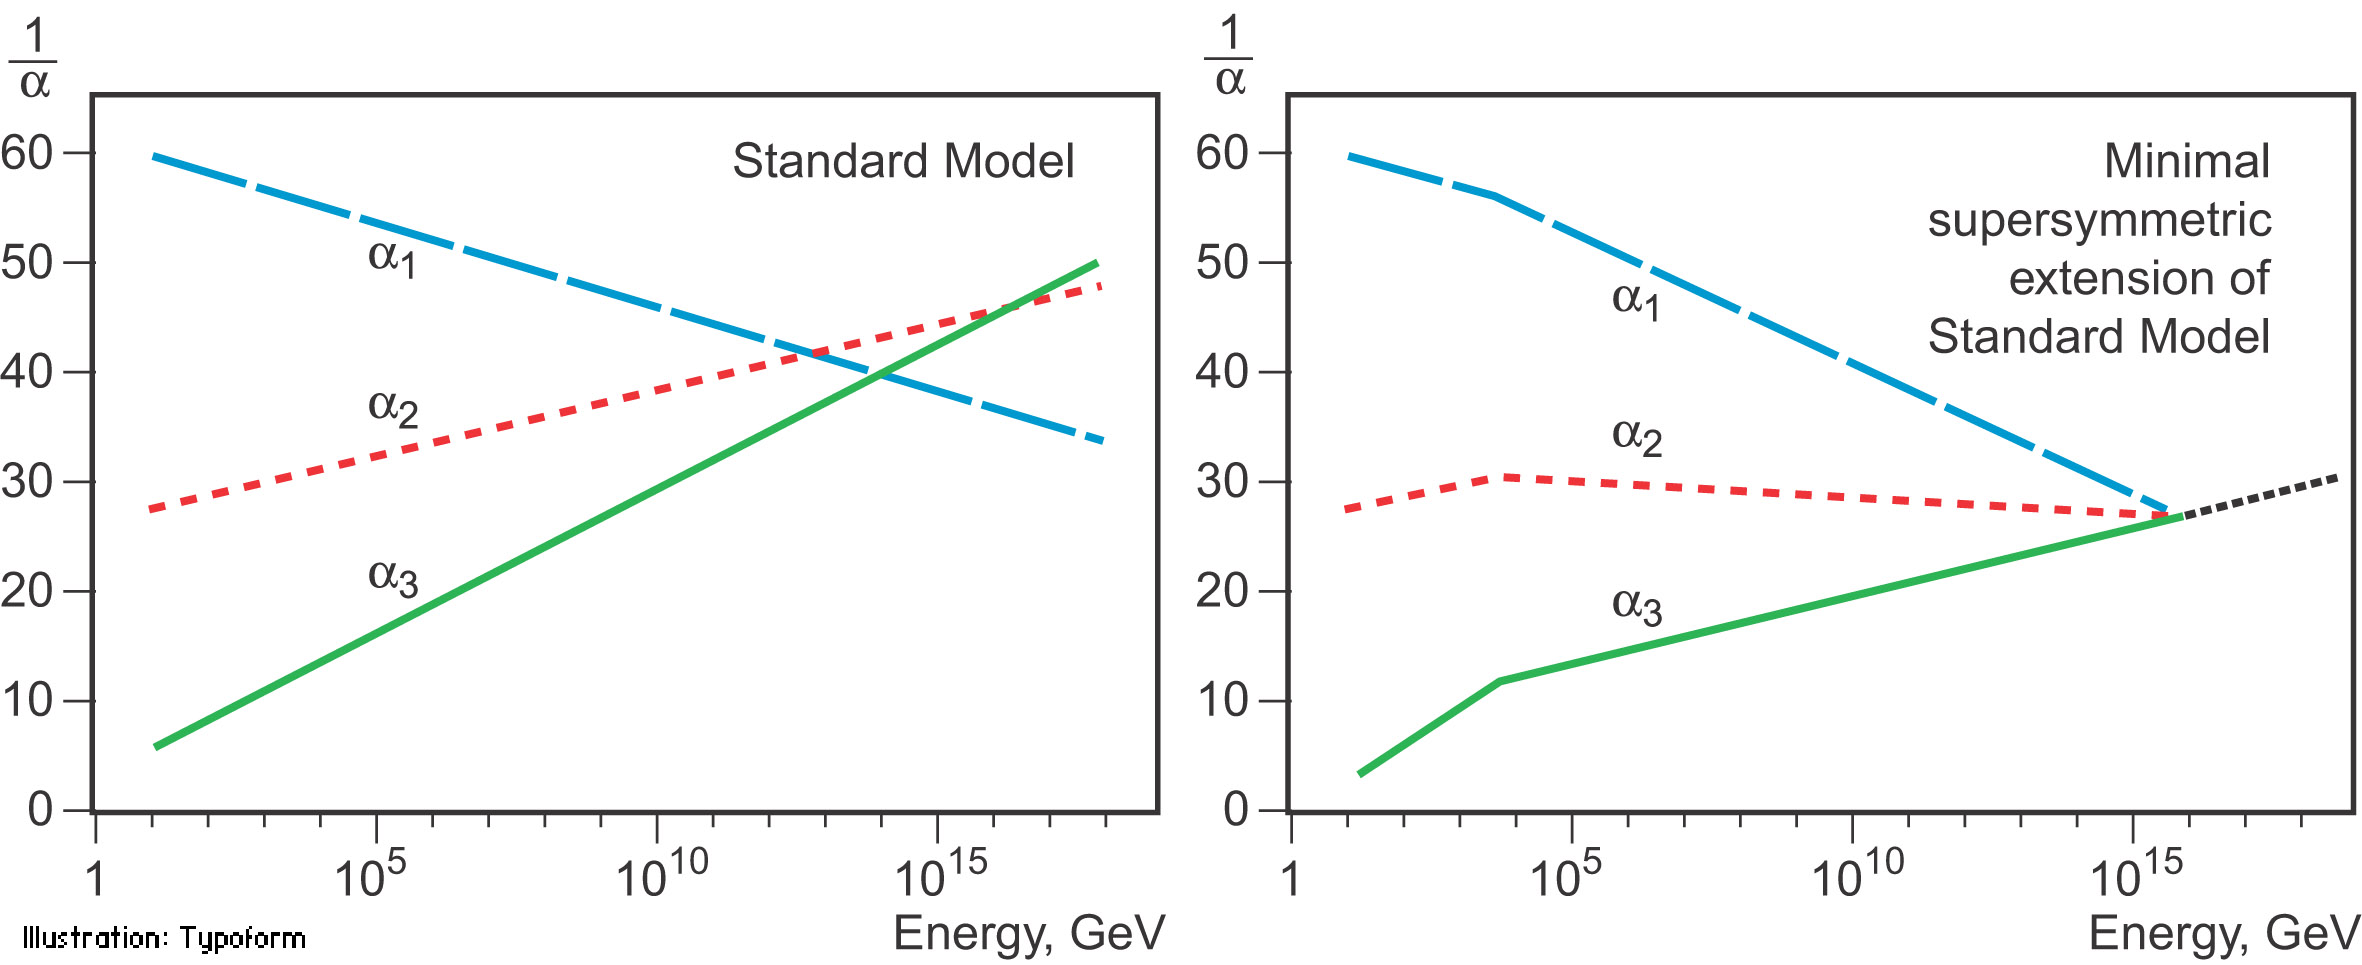
\includegraphics[width=0.65\textwidth,]{figures/phypub4highen.jpg}
       \caption{The coupling constant values for the electromagnetic (blue), weak (red), 
       and strong (green) interactions as a function of energy scale for the SM (left) and the simplest 
       supersymmetric extension of the SM (right).}
    \label{fig:runningConstants}
  \end{center}
\end{figure}

Supersymmetry (SUSY) theory is an extension of the SM. For each fermion (or boson) in
the SM, a new supersymmetric boson (or fermion) is introduced. Theories that incorporate 
supersymmetry (SUSY) introduce a new symmetry between bosonic and fermionic states. 
Any theory invariant under a transformation between these states is called 
supersymmetric~\cite{ramond1999journeys}.\\
\indent A strong motivation for such a theory is that, if the energy scale is low enough, the 
divergent terms to the Higgs mass is removed; the corrective terms from fermionic loops are canceled by 
opposite-sign supersymmetric bosonic loop terms and vice versa. Another attractive feature
of the theory is that, at large energy scales, i.e. energies present in the early universe, 
values of the coupling strengths for the electromagnetic, weak, and strong interactions converge 
to a single value, hinting at a possible grand unified theory of the interactions~\cite{wess1992supersymmetry}. 
This unification is not achieved in the Standard Model. Figure~\ref{fig:runningConstants} show the 
dependence of the coupling constants of the three interactions as a function of energy scale 
for the SM (left) and the simplest supersymmetric extension of the SM (right). Furthermore,
SUSY theories provide a lightest supersymmetric particle (LSP) which does not decay and only 
interacts weakly. This LSP could be a constituent of dark matter.\\
\indent The SM particle and its supersymmetric partner are identical in every quantum number except spin. 
The spin of the supersymmetric is derived from the spin of the SM particle $S_{m}$ by 
subtracting $\frac{1}{2}$ the exception being the Higgs boson which $\frac{1}{2}$ is added
to the spin. The superpartners of the leptons (l) are called sleptons $\tilde{l}$. 
Squarks $\tilde{q}$ are the partners of the quarks q. Gluinos $\tilde{g}$ are partners
of the gluon g. In contrast to the one Higgs doublet in the SM (Eqn.~\ref{eq:higgs-field}), 
two doublets are needed in SUSY. One of the doublets can only give mass to up-type quarks because of
the Yukawa coupling it possesses, and the other doublet gives mass to the down-type 
quarks and to the charged leptons. These two doublets have eight degrees of
freedom three of which are absorbed by the gauge bosons of the weak interaction
just as in the SM resulting in five physical higgs bosons.
The neutral superpartners of the gauge boson fields, Bino $\widetilde{B}$ and Wino $\widetilde{W}^0$, mix
with the neutral $\widetilde{W}^0$ to form the four mass eigenstates of the so-called neutralinos 
$\widetilde{\chi}^0$. The charged gauginos and Higgsinos mix to create charginos $\widetilde{\chi}^{\pm}$.
The sparticles and their the SM partners are summarized in Table~\ref{tab:sparticleTable}.

\begin{figure}[h!t]
  \begin{center}
       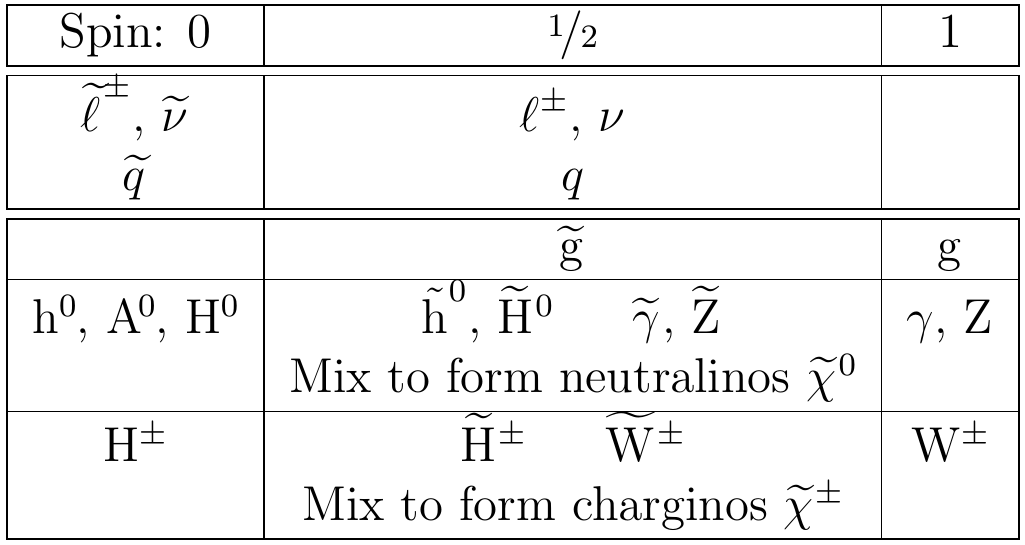
\includegraphics[width=0.45\textwidth,]{figures/sparticleTable.png}
       \caption{The extended particle spectrum of SUSY theories. For every boson a fermion
       is introduced, and vice versa. Additionally a two Higgs doublet model is necessary 
       leading to five physical Higgs bosons.}
    \label{tab:sparticleTable}
  \end{center}
\end{figure}

It is important to note that from the start, SUSY theories were introduced as theories with a 
broken symmetry. Since supersymmetric particles had not been discovered (and still haven't been in fact), 
it was imposed, via a broken symmetry, that the mass of the sparticles had to be higher than 
those of their SM partners. But in order to keep the cancellation of the divergent corrections to 
the Higgs mass, this break in symmetry needs to happen at a sufficiently low energy scale, 
i.e. $\mathcal{O}$(1~TeV)~\cite{ramond1999journeys}.\\
\indent In the SM, the baryon number B and the lepton number L are conserved since no possible 
renormalizable Lagrangian terms can introduce such violation. In contrast for the superpotential in 
SUSY an additional multiplicative quantum number is introduced to ensure the conservation of B and L, the so-called R-parity:

\begin{equation}
\label{eq:r-par}
R = \left(-1\right)^{3B+L+2s},
\end{equation}

where s is the spin of the particle. R = 1 for ordinary standard model particles and R = -1 for SUSY sparticles.
In the construction of the simplest implementation of SUSY consistent with the SM, called the Minimal 
Supersymmetric Standard Model (MSSM), R-parity is made to be conserved. This conservation has some significant consequences:

\begin{itemize}
\item{Every supersymmetric particle will eventually decay into the LSP, or at least an odd
number of LSPs}
\item{The LSP is a stable, i.e. its decay would be R-parity violating}
\item{SUSY particles must be produced in pairs}
\end{itemize}

Although there is still interest in R-parity violating theories and experimental searches are still
very much active, R-parity conserving theories are usually preferred. One reason being that the decay of 
the proton has not been observed, which an unconstrained R-parity violating theory predicts. The 
phenomenology of R-parity violating models is quite different because the LSP decays can decay into SM 
particles. The search strategy of this analysis and the SUSY models used to interpret the results assume 
R-parity conservation.

\subsection{Experimental signature}
\label{sec:signature}

Color confinement in QCD prohibits the isolation of quarks~\cite{Ellis:1991qj} 
and as such, when a high energy quark is produced, e.g. 
from a collision of other particles, it quickly fragments into a 
color-neutral hadron. If the quarks in the hadron have enough energy, 
they fragment again into other hadrons. This hadronization process 
continues until the resulting particles are of low enough energy that it
is no longer energetically favorable to fragment. The hadronic shower of
particles can be clustered into objects called ``jets''. A simulation 
of such a jet is shown in Figure~\ref{fig:jets}.  

\begin{figure}[h!t]
  \begin{center}
       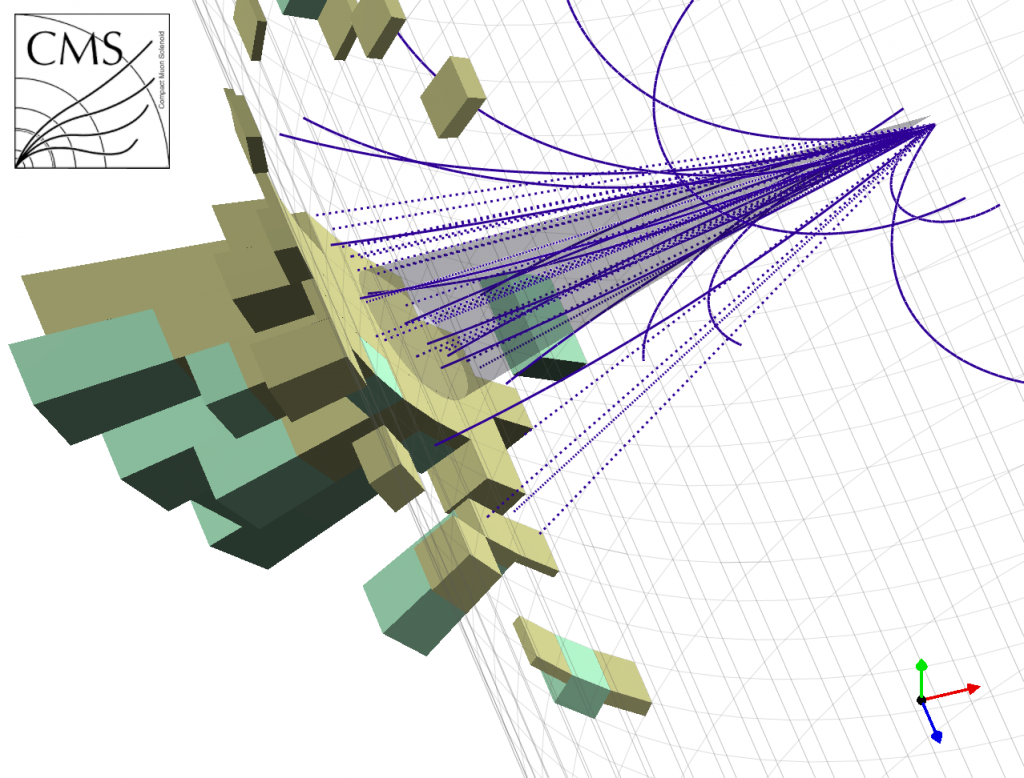
\includegraphics[width=0.45\textwidth,]{figures/JetConeAndPFJet.png}
       \caption{A simulation of a hadronized quark in the CMS detector. The
       resulting particles from hadronization are grouped into a jet (gray cone). }
    \label{fig:jets}
  \end{center}
\end{figure}

In this analysis, a search for excess in events consisting of jets and 
missing energy is conducted. This final state is expected when pairs of
heavy squarks or gluinos are produced and decay hadronically to SM quarks,
gluons, and neutralino, which escape the detector leaving only a signature
of missing energy.
%Such an excess would not directly validate a 
%supersymmetric extension of the Standard Model, since other interpretation are 
%possible, but nonetheless supersymmetry provides a extensive framework for interpretation. 
The full unconstrained SUSY theory is parametrized by over 100 variables, representing 
masses, phases and mixing angles, but it can be simplified. These simplified supersymmetric 
models (SMS) are limits of more general new-physics scenarios, where all but a few 
particles are integrated out~\cite{Alves:2011wf}.\\
%Since new physics is thought to potententially arise at the scale of $\mathcal{O}$(1~TeV), 
\begin{figure}[ht!]
  \begin{center}
    \subfigure[\label{fig:feyn_t2tt}]{
      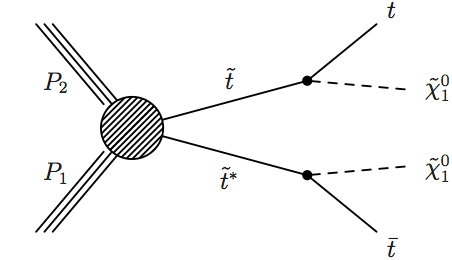
\includegraphics[width=0.45\textwidth,]{figures/T2tt}
    } 
    \subfigure[\label{fig:feyn_t2cc}]{
      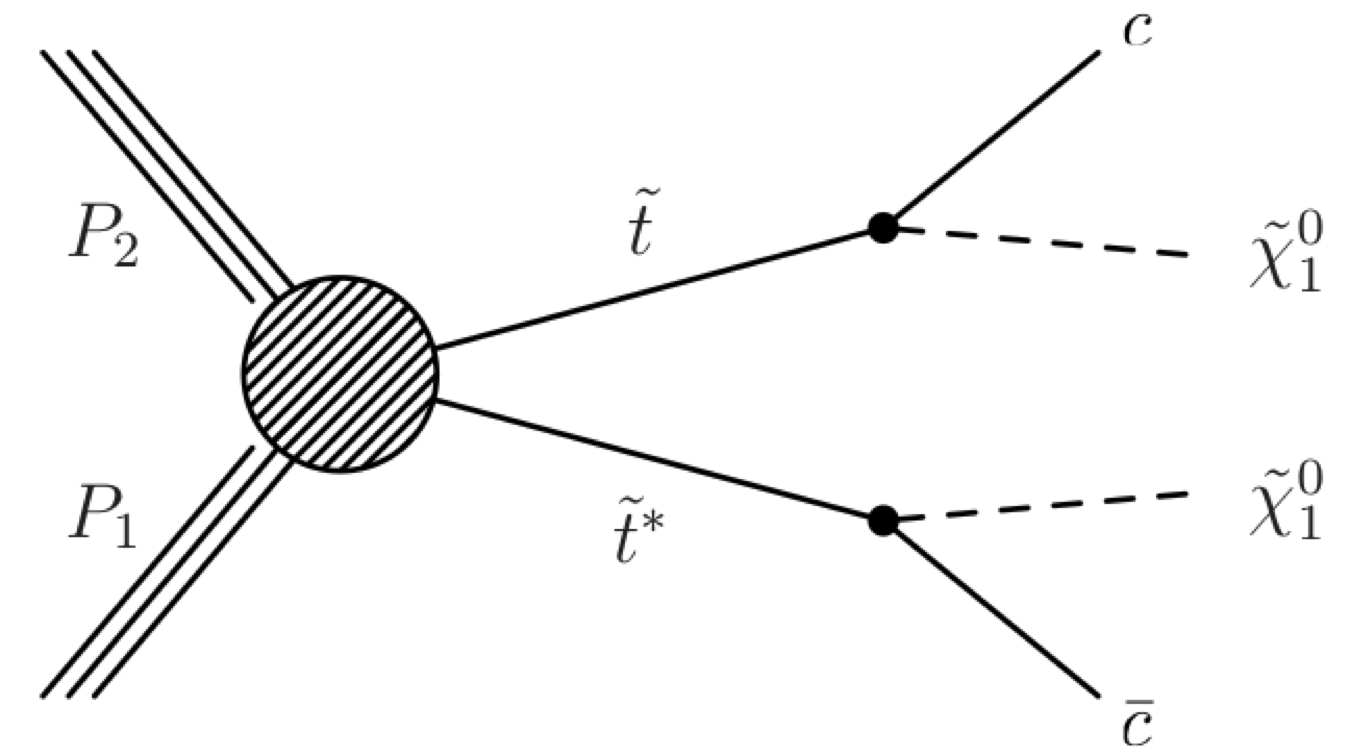
\includegraphics[width=0.45\textwidth,]{figures/T2cc}
    } \\
      \caption{Two Feynman diagrams depicting the top squark production
      and decay, in which P represents a proton, $t$ a top quark, $c$ a charm
      quark, $\st$ a top squark, \chiOnez a neutralino.}
    \label{fig:feynman_sms}
  \end{center}
\end{figure}

\indent Some of the earliest SUSY searches at the LHC focused on 
looking for SUSY in the production and decay of gluinos and first- and 
second-generation squarks. The idea being that these processes have the highest 
theoretical rate of production at the LHC (Fig.~\ref{fig:crossSec}) and could provide the first hints of a 
supersymmetric extension to the SM. After the first three LHC runs and over $20~\fbinv$ of
collected data, the current situation is that gluino masses below $1.1~\TeV$ and first- and 
second-generation squark masses below $800~\gev$ have been excluded by the CMS~\cite{cms-susy} 
and ATLAS~\cite{atlas-susy}. As these searches, within the ability of the experiment and beam energy,
have been exhausted, this analysis chose to focus on the search for third-generation 
squarks, more specifically the top squark.\\
\indent Such a search presents some challenges. Direct production of top squark pairs at hadron 
colliders is suppressed with respect to first generation squarks by a factor of $\sim100$. This is 
due to the negligible amount of third generation quarks in the colliding protons. Moreover, at 
the LHC, there is a very large background of top quark pair production, complicating the search for an excess.
Low-energy SUSY (i.e. at the TeV-scale) is often motivated as a solution to 
stabilize quadratic divergences in radiative corrections to the Higgs boson mass. In this
context, the most relevant terms for SUSY phenomenology arise from the interplay between 
the mass of the top squark and its coupling to the Higgs boson~\cite{Agashe:2014kda}. 
Due to the large top quark mass, significant mixing between the left- and right-handed squark
is expected, leading to two squark mass eigenstates. In the MSSM, the lightest top squark
can have the mass of the top quark, or even lower~\cite{Martin:1997ns}.\\
\indent This relatively low mass is a motivation to interpret the results of this 
analysis in two decay channels of the direct pair-produced top squark. 
In the first channel, where the top squark decays to a top quark, provides the highest reach 
in probing the mass of the top squark. The decay channel populates the right-most region of the 
neutralino-stop mass plane in Figure~\ref{fig:mStop_mLsp}.
The second decay scenario has only been recently pursued at the LHC. It puts 
the mass difference between the top squark and the neutralino at 80~\GeV or 
less, resulting in the top squark decaying directly into a charm quark. 
The corresponding final state is characterized by the presence of two jets from 
the hadronization of the charm quarks and escaping energy from two undetected LSPs.
The small mass difference between the top squark and the LSP in this model has consequences on the 
identification of such events and those details are discussed in Section~\ref{sec:signal}.
The decay channel populates the strip adjacent of the shaded region in Figure~\ref{fig:mStop_mLsp}.
Figure~\ref{fig:feynman_sms} shows the schematic diagrams of these two decay channels.

\begin{figure}[ht!]
  \begin{center}
      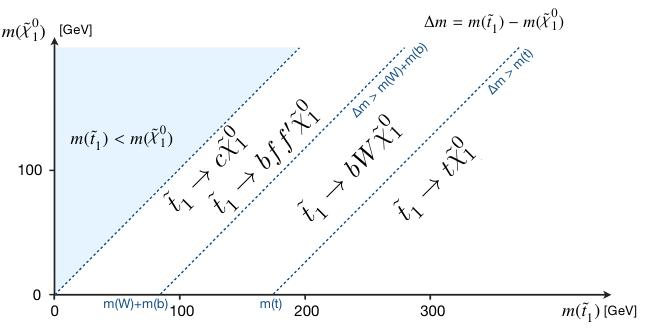
\includegraphics[width=0.65\textwidth,]{figures/mstop_mLSP_plane.jpg}
      \caption{The neutralino-stop mass plane spanned by the potential decay channel from 
      direct stop productions.}
    \label{fig:mStop_mLsp}
  \end{center}
\end{figure}
